% ============================== Header ==============================
\documentclass{article}
\usepackage[a4paper, top=8mm, bottom=8mm, left=8mm, right=8mm]{geometry}
\usepackage[most]{tcolorbox}
\usepackage[hidelinks]{hyperref}
\usepackage[defaultfam,tabular,lining]{montserrat}
\usepackage{dirtytalk}
\usepackage{fontawesome5}
\usepackage{setspace}

\begin{document}

% ============================== Global settings ==============================
\setlength{\parindent}{0mm} % No paragraph indent
\pagenumbering{gobble} % No page numbering
\setstretch{1.5} % Set line spacing
\large % Set find size

% ============================== Custom commands ==============================
\definecolor{custom_blue}{RGB}{2,132,199}
\definecolor{linkedin_blue}{RGB}{10,102,194}
\newcommand{\NameText}[1] {{\huge \textbf{#1}}}
\newcommand{\HighlightedText}[1] {{\large \textbf{#1}}}
\newcommand{\Section}[1]{
    \vspace{2mm}
    \HighlightedText{#1}
    \vspace{1mm}
    {\color{custom_blue} \hrule}
    \vspace{3mm}
}
\newcommand{\ItemizeSection}[1]{
    \vspace{2mm}
    \HighlightedText{#1}
    \vspace{1mm}
    {\color{custom_blue} \hrule}
}

% ============================== Name and Contact ==============================

\begin{tcolorbox}[sharp corners=all, colback=custom_blue, coltext=white, frame empty, left=2mm, right=2mm, top=2mm, bottom=2mm]

    \noindent \begin{minipage}{0.7\textwidth}
        \NameText{Kyrylo Sovailo}

        \faAt \hspace{0.0mm} \href{mailto:k.sovailo@gmail.com}{\underline{k.sovailo@gmail.com}}

        \faPhone* \href{tel:+4917635479038}{\underline{01763 5479038}}

        \faEnvelope \hspace{0.0mm} Pallaswiesenstr. 39, 64293 Darmstadt

        \faGithub \hspace{0.0mm} \href{https://github.com/kyrylo-sovailo}{github.com} \hspace{5.0mm} \faLinkedin \hspace{0.0mm} \href{https://linkedin.com/in/kyrylo-sovailo-19b4541b9}{linkedin.com}
    \end{minipage}
    \begin{minipage}{0.29\textwidth}
        \centering
        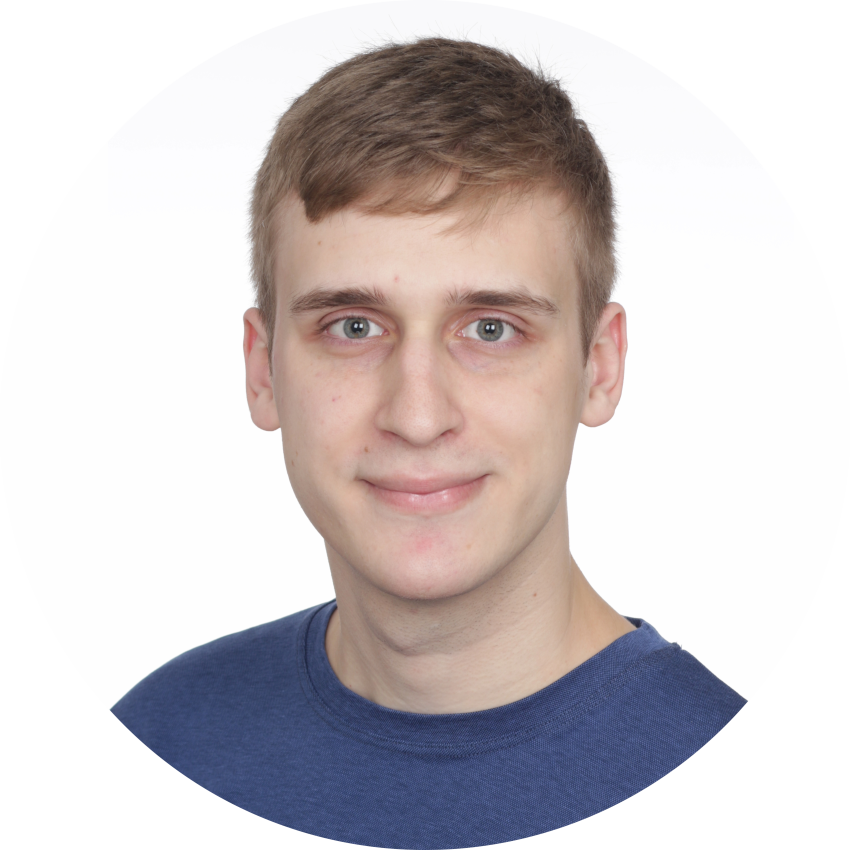
\includegraphics[width=3.5cm]{Photo_compressed_round.png}
    \end{minipage}
\end{tcolorbox}
\setstretch{0.0}

% ============================== Education ==============================
\ItemizeSection{Ausbildung}
\begin{itemize}
    \item[$\bullet$] \HighlightedText{TU Darmstadt} \hfill \HighlightedText{2023 -- 2025}

    Computational Engineering (CE), Master

    \item[$\bullet$] \HighlightedText{RWTH Aachen University} \hfill \HighlightedText{2018 -- 2023}

    Computational Engineering Science (CES), Bachelor

    \item[$\bullet$] \HighlightedText{Studienkolleg an Freier Universität Berlin} \hfill \HighlightedText{2017 -- 2018}

    Technischer Kurs (T-Kurs)

    \item[$\bullet$] \HighlightedText{Technisches Lyzeum} \hfill \HighlightedText{2010 -- 2017}

    Technisches Lyzeum von Nationaler Technischer Universität der Ukraine \say{Kiew Polytechnisches Institut}
\end{itemize}

% ============================== Professional background ==============================
\ItemizeSection{Professioneller Hintergrund}
\begin{itemize}
    \item[$\bullet$] \HighlightedText{Masterarbeit an SIM von TU Darmstadt} \hfill \HighlightedText{Februar 2025 -- September 2025}
    \begin{itemize}
        \item[$\circ$] Thema: Integration von räumlicher Wahrnehmung in embeddings-basierte Anomalieerkennungsmethoden für die automatisierte industrielle Inspektion
        \item[$\circ$] Entwicklung von Algorithmen auf Basis von ViT-Modellen (torch, transformers, Python)
    \end{itemize}

    \item[$\bullet$] \HighlightedText{Hilfskraft an BMLS von Goethe Universität Frankfurt} \hfill \HighlightedText{Juni 2023 -- Juli 2024}
    \begin{itemize}
        \item[$\circ$] Entwickung eines Slicer-Programms (C++, C\#, Slic3r)
        \item[$\circ$] Programmierung des Controllers von einem Bio-3D-Drucker (C++, Arduino)
    \end{itemize}

    \item[$\bullet$] \HighlightedText{Bachelorarbeit an DSME von RWTH Aachen} \hfill \HighlightedText{Juni -- September 2022}
    \begin{itemize}
        \item[$\circ$] Thema: Balancierung eines 2D inverses Pendels mit Franka Panda Roboterarm
        \item[$\circ$] Entwicklung von Algorithmen für inverse Kinematik, inverse Dynamik und Robotersteuerung (ROS, C++, Python)
    \end{itemize}

    \item[$\bullet$] \HighlightedText{Praktikum an Continental AG} \hfill \HighlightedText{März 2022 -- Mai 2022}
    \begin{itemize}
        \item[$\circ$] Aufbau eines Tools zur Erstellung von C aus CAN-Datenbanken (Python, C, CAPL)
        \item[$\circ$] Aufbau einer Toolchain für Programmierung von V850 Mikrokontroller (CMake, Python)
    \end{itemize}

    \item[$\bullet$] \HighlightedText{Hilfskraft an DSME von RWTH Aachen} \hfill \HighlightedText{April -- Dezember 2021}
    \begin{itemize}
        \item[$\circ$] Entwicklung eines Steueralgorithmus für einen Franka Panda Roboterarm (Echtzeit Linux, C++, Python)
        \item[$\circ$] Implementierung einer Simulation des Roboters (C++, Gazebo)
    \end{itemize}
\end{itemize}

% ============================== Skills ==============================
\ItemizeSection{Qualifikationen}
\begin{itemize}
    \item[$\bullet$] Kenntnisse von C, C++, C\#, Python, Matlab/Simulink, git, CMake, ROS, \LaTeX

    \item[$\bullet$] Erfahrung mit eingebetteten Systemen: AVR, ARM (inkl. Raspberry Pi, NVidia Jetson)

    \item[$\bullet$] Erfahrung mit stationären sowie mobilen Robotern

    \item[$\bullet$] Kenntnisse von Autodesk Inventor, FreeCAD, KiCAD (inkl. Kenntnisse von Elektronik)

    \item[$\bullet$] Fortgeschrittener Umgang mit Linux (inkl. Kernelkonfigurierung)
\end{itemize}

% ============================== Other ==============================
\Section{Sonstiges}

\hspace{2.5mm} Ich habe einen Github Account mit persönlichen Projekten: \hspace{0.0mm} \faGithub \hspace{0.0mm} \href{https://github.com/kyrylo-sovailo}{github.com/kyrylo-sovailo}

\hspace{2.5mm} Im 2017 gewann ich eine Bronzemedaille bei der Internationalen Physikolympiade.

\end{document}
